
El fichero de definición de una imagen Docker se le nombra por defecto Dockerfile.
Expresa la imagen base desde la que se parte, el fichero diseñado usa un sistema operativo debian, y se procede a ejecutar los distintos pasos de instalación de dependencias que se requieren para construir el contendor.
En un mismo fichero Dockerfile existen distintos stages.
Un stage es cada conunto de pasos diferenciados por un nombre.
A la hora de levantar el contenedor se puede seleccionar el requerido.
Esto es útil para, en un mismo fichero, especificar si queremos instalar las dependencias para desarrollo o producción.
Así se especifican y ahorran los elementos comunes, que de otro modo habrían de duplicarse y mantener en ficheros separados.
Los stages diseñados son: base, dev, compile y prod.

En la base se instalan los elementos comunes.
Si se especifica dev entonces se instala Golang, el debugger Delve, un usuario para evitar el uso de sudo dentro dicho container y distintas utilidades generales como git, vim como editor de textos y fish como terminal.
Si se construye mediante la etiqueta \textit{compile} se evita la instalación de los elementos de desarrollo y sólo instalamos golang para poder compilar el código.
En prod se usa esa fase primero para compilar.
Luego se parte de la base en limpio y se crea un contendor con el ejecutable en su interior.
Ahorrando espacio en el contenedor.
Estos pasos pueden apreciarse en la~\cref{fig:dockerfile}.

\begin{figure}[H]
    \centering
    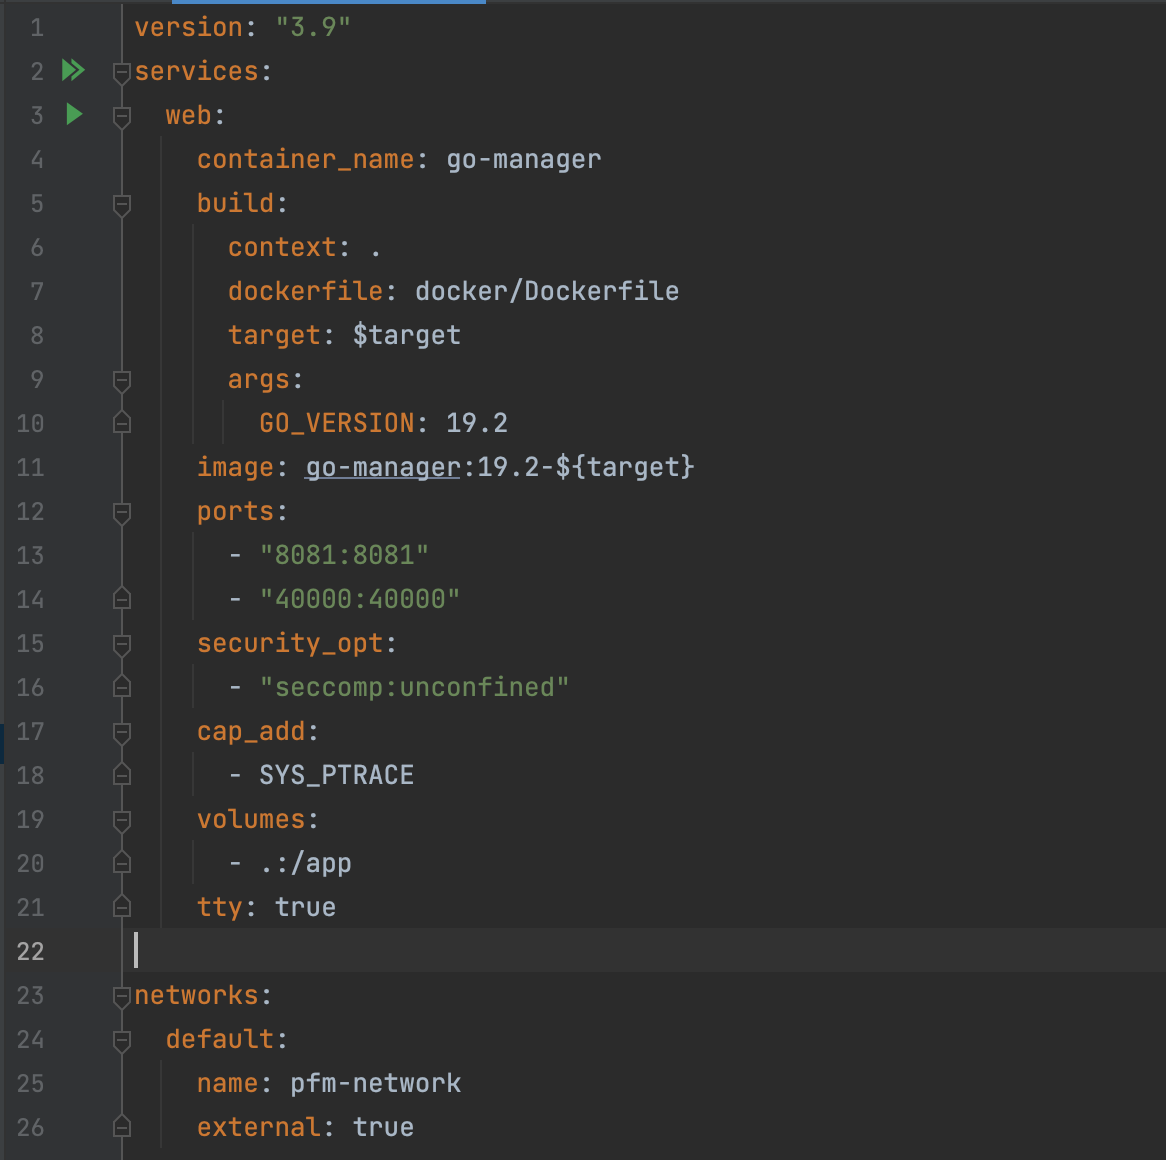
\includegraphics[scale = 0.6]{part/Proyecto_ejecutivo/memoria_constructiva/docker/docker-compose}
    \caption{Docker-compose.yml para cada proyecto golang: Manager, client y control}\label{fig:dockercompose}
\end{figure}

\begin{figure}[H]
    \centering
    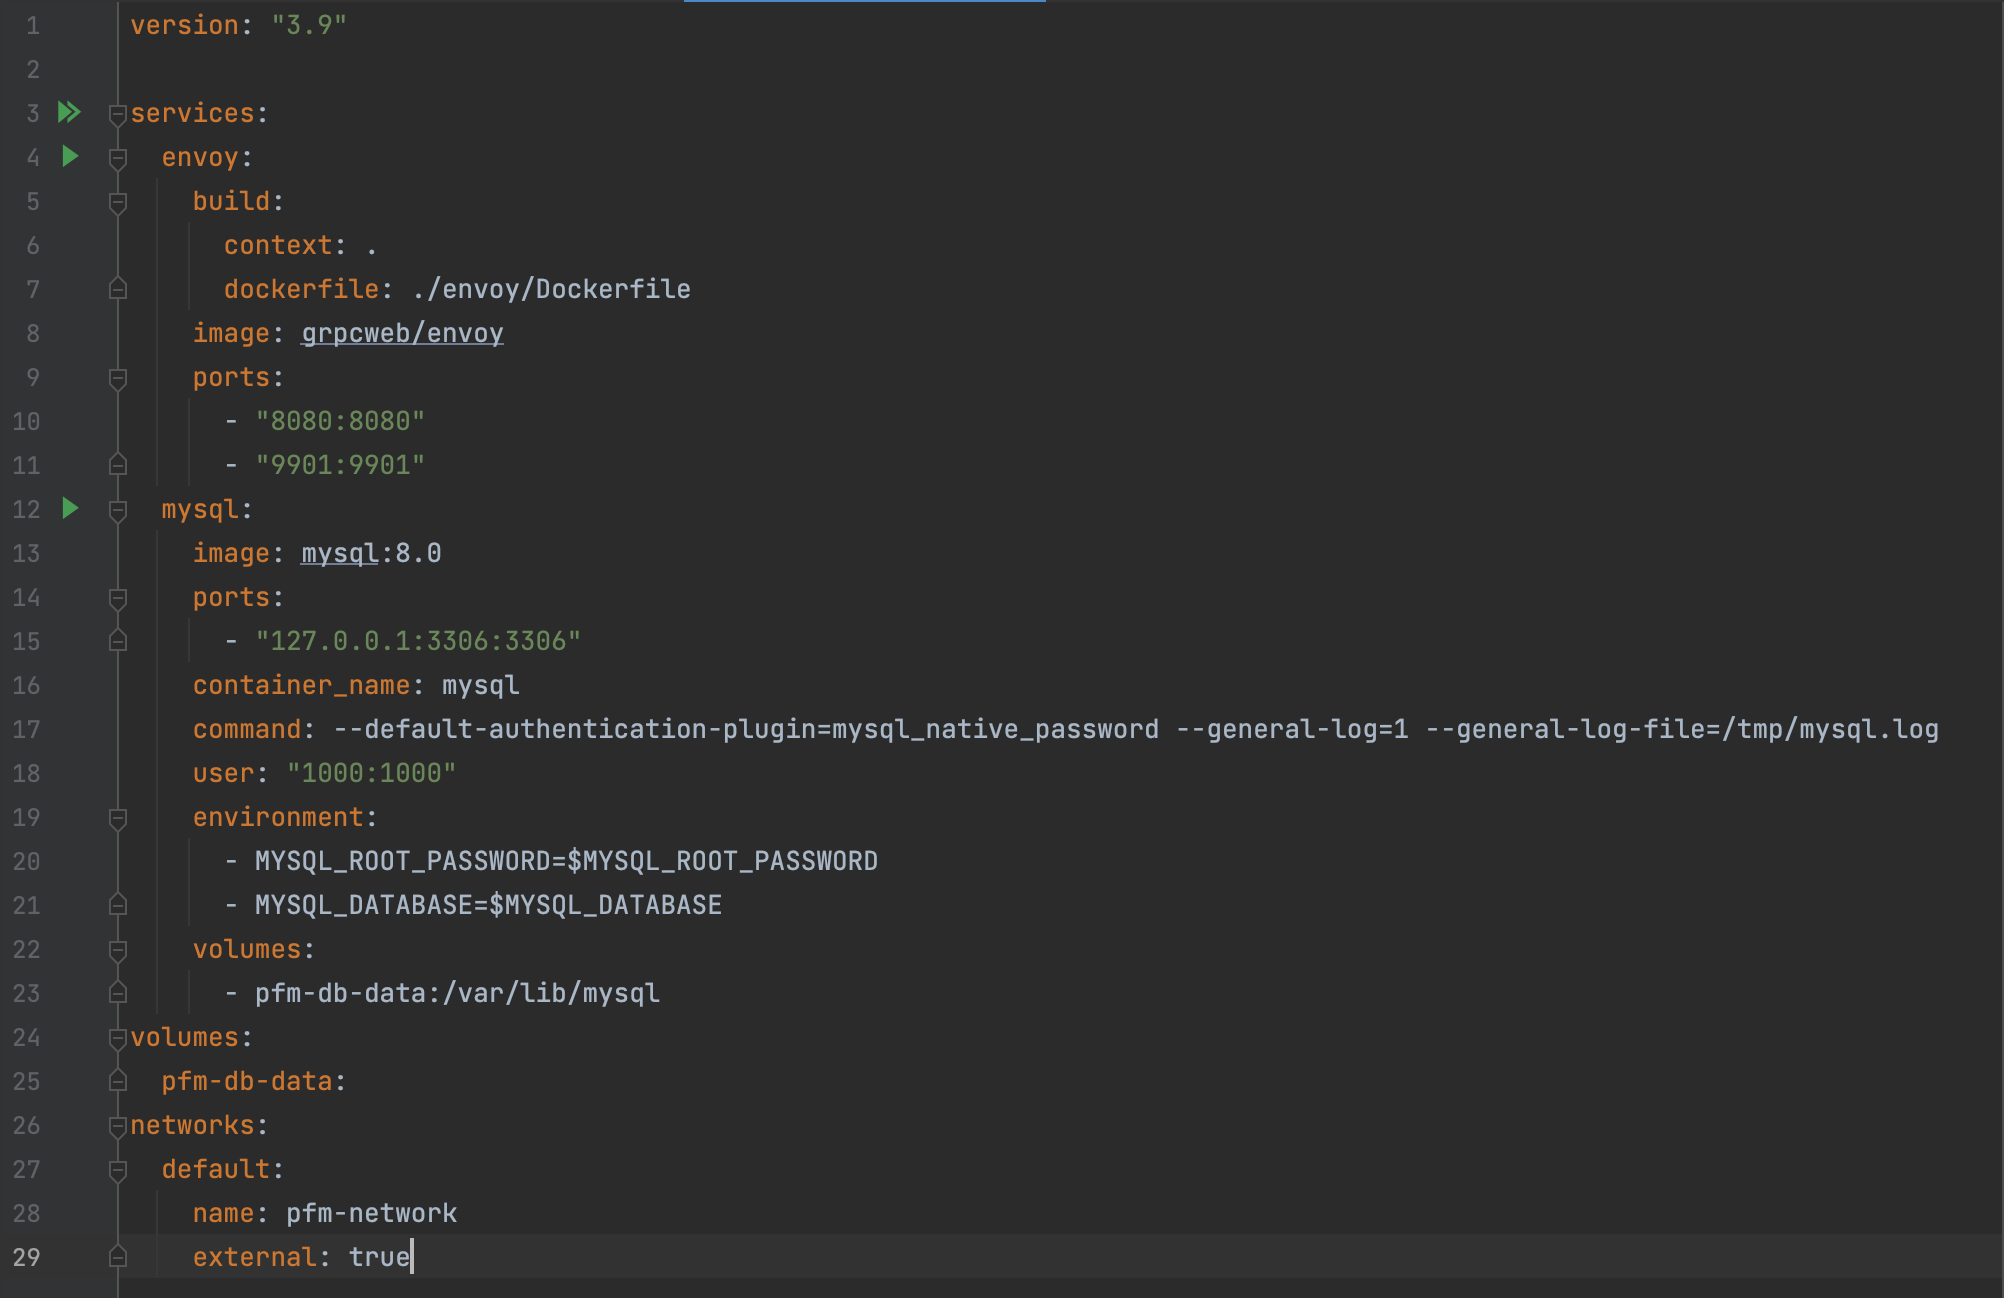
\includegraphics[scale = 0.3]{part/Proyecto_ejecutivo/memoria_constructiva/docker/docker-compose-gen}
    \caption{Docker-compose.yml definicion de base de datos y proxy RPC}\label{fig:dockercomposegen}
\end{figure}

La infraestructura consta además de una red para hacer visible los contenedores entre si: Manager, clients, base de datos y el proxy para el RPC. La estructura se especifica en un archivo docker-compose.yml .~\cref{fig:dockercompose}.
Habrá un docker-compose.yml aparte para el proxy y la base de datos.~\cref{fig:dockercomposegen}

\begin{figure}[H]
    \centering
    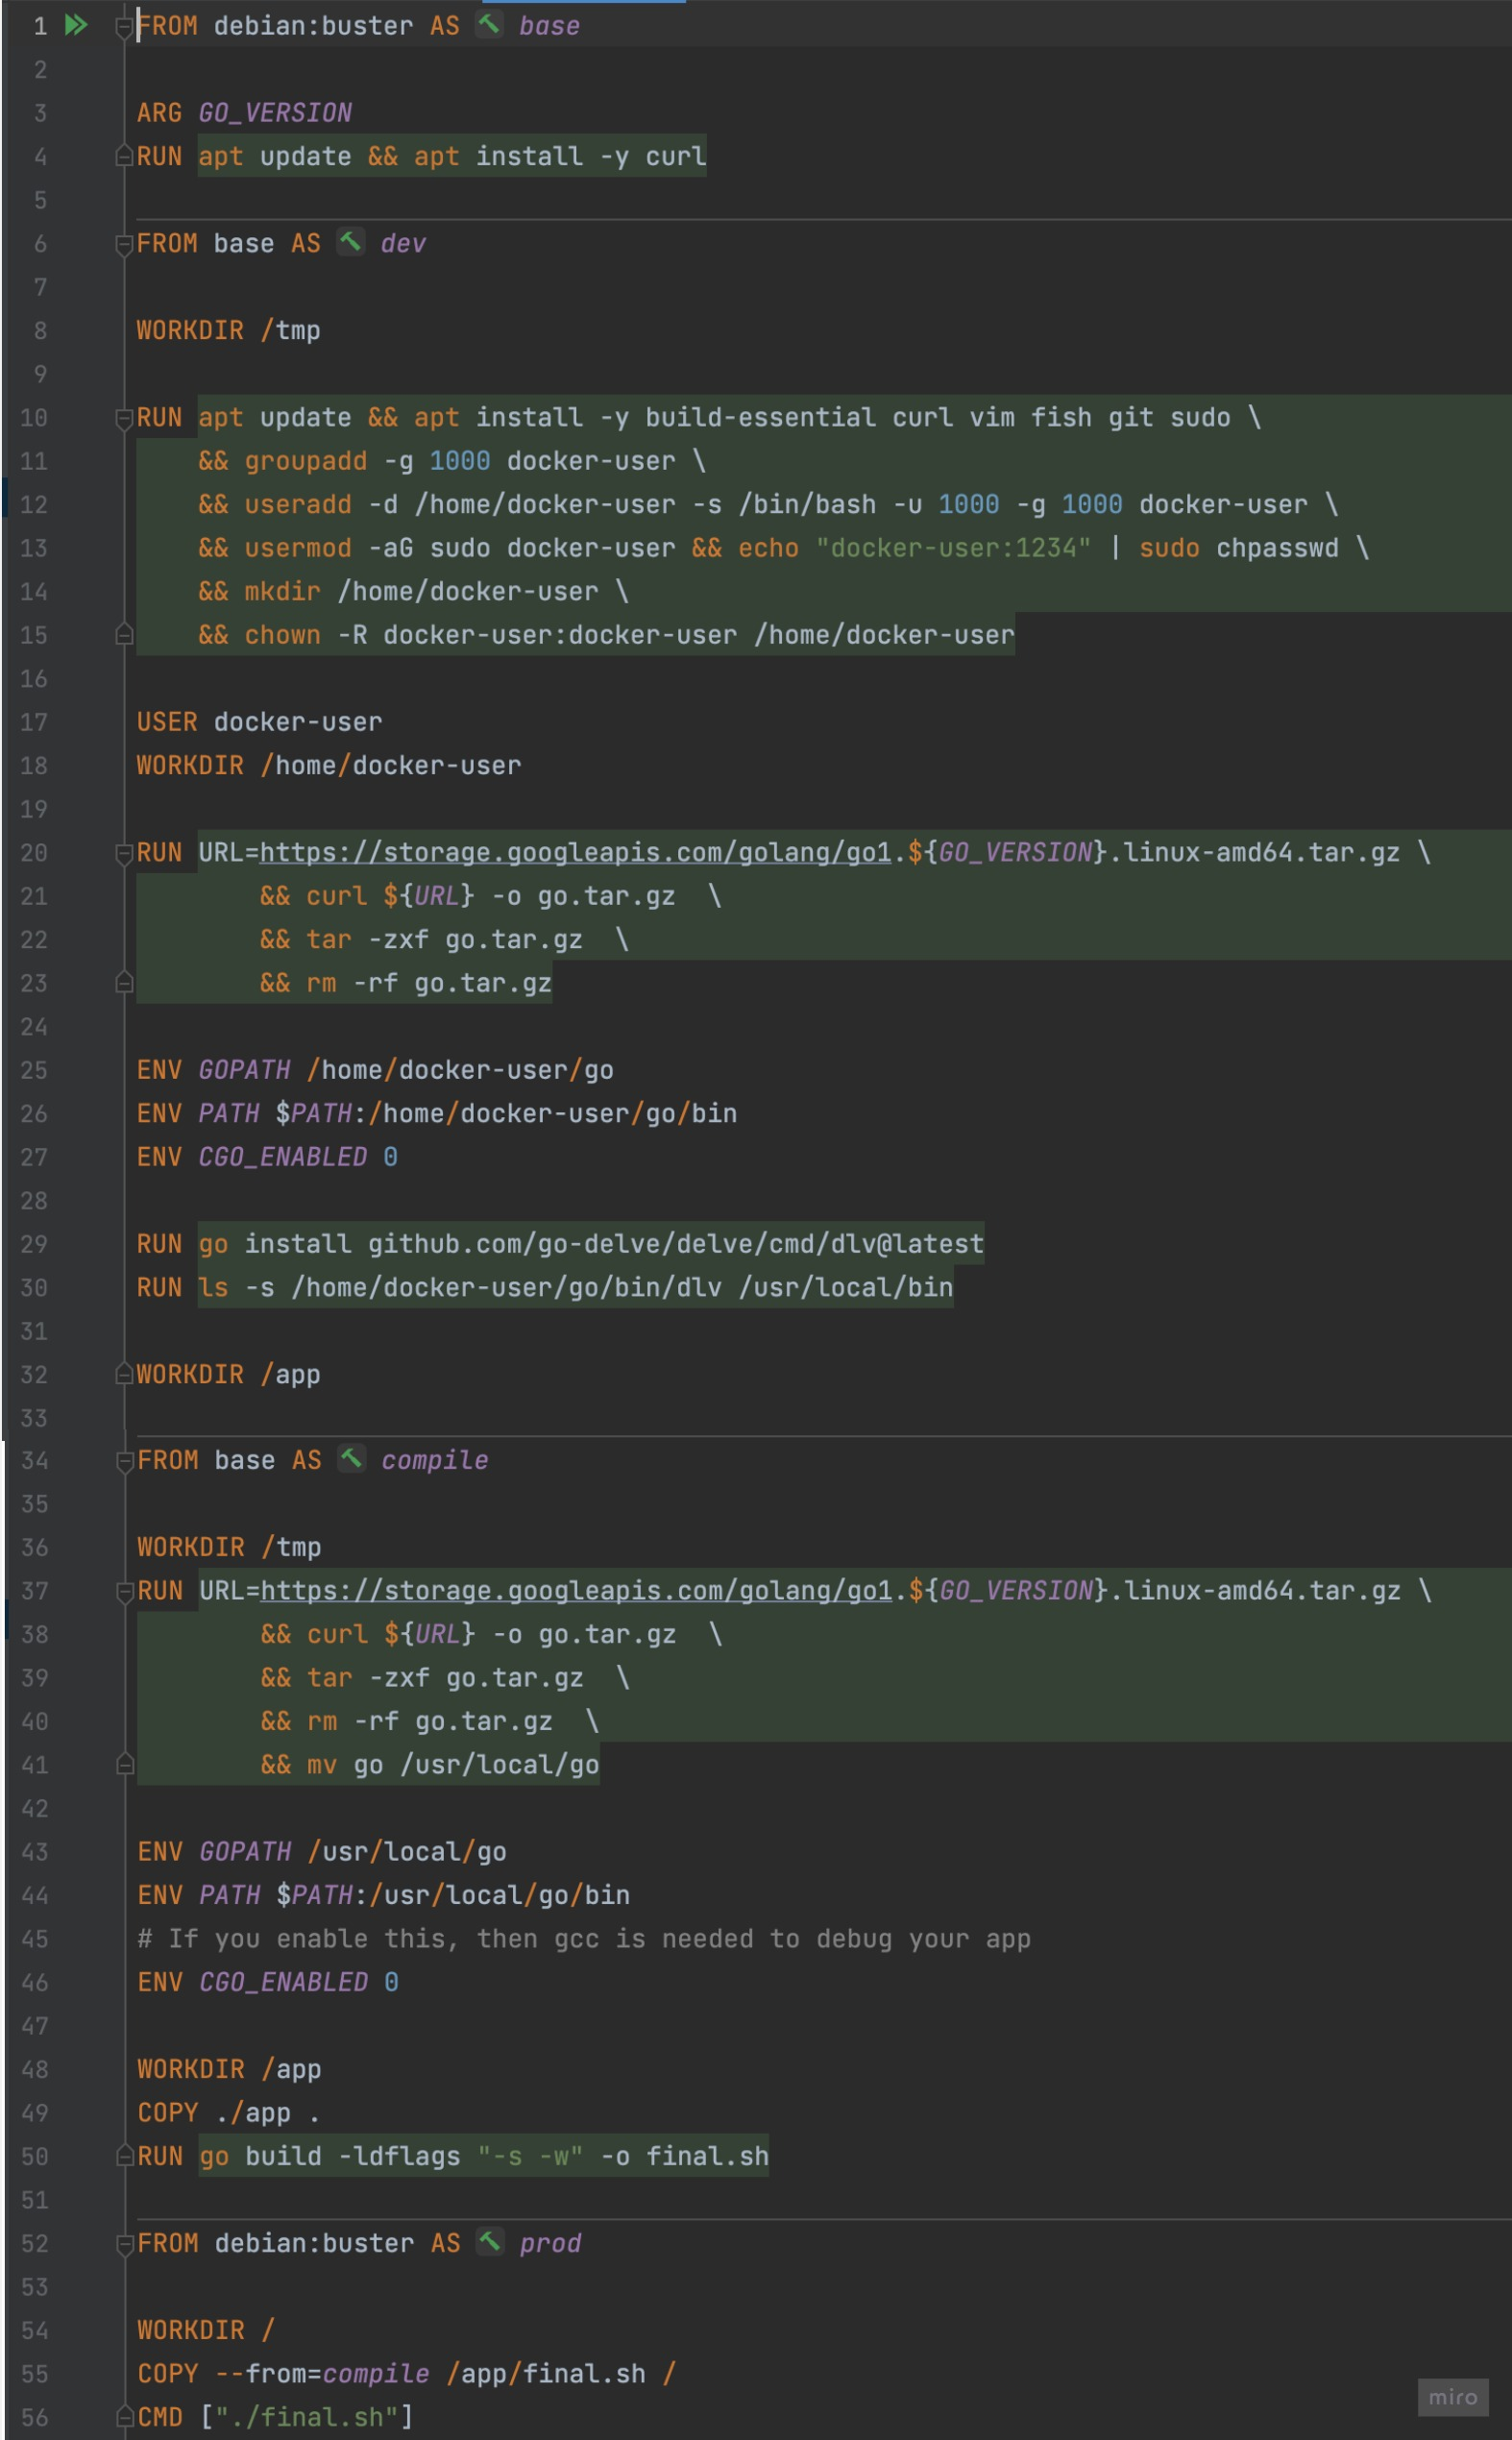
\includegraphics[scale = 0.25]{part/Proyecto_ejecutivo/memoria_constructiva/docker/PFM - Dockerfile}
    \caption{Dockerfile.yml}\label{fig:dockerfile}
\end{figure}